\documentclass[12pt,a4paper,notitlepage]{article}

\usepackage{fontspec}
\usepackage{minted}
\usepackage{xunicode}
\usepackage{amsmath}

%\usepackage[pdftex]{graphicx,color}
%\usepackage[utf8x]{inputenc}
%\usepackage{amssymb,amsmath}
%\usepackage{wasysym}
%\usepackage[T1]{fontenc}
%\usepackage{ucs}
%\usepackage{eurosym}

\usepackage{ngerman}
\usepackage{setspace}
\usepackage{cite}
\usepackage{fancybox}
\usepackage[notree,order=word,acronym]{glossaries}
\usepackage{tabularx}
\usepackage{multicol}
\usepackage{hyperref}
\usepackage{todo}
\usepackage{pdflscape}

\usepackage[a4paper,textwidth=17cm, top=2cm, bottom=3.5cm]{geometry}

%\usepackage{url}
%\usepackage{fourier}
%\usepackage{marvosym}
\definecolor{p-green}{rgb}{0.12,0.57,0.11}
\newcommand{\bitem}{\item[--]}
\newcommand{\litem}[2]{\item[#1 --] #2}
\newcommand{\blitem}[3]{\item[#1 --] \texttt{#2} -- #3}
\newcommand{\gfo}{\grqq\ }
\newcommand{\gfu}{\glqq}
\newcommand{\zquote}[2]{\glqq #1\grqq\ (Z.\ #2)}
\newcommand{\pquote}[1]{\glqq #1\grqq}
\newcommand{\nquote}[2]{#1: \glqq #2\grqq}
\newcommand{\nwquote}[3]{#1 -- \emph{#2}: \glqq #3\grqq}
\newcommand{\nwyquote}[4]{#1 -- \emph{#2} (#3): \glqq #4\grqq}
\newcommand{\diff}{\mathrm{d}}
\renewcommand{\abstractname}{}
\definecolor{orange}{rgb}{1,0.6,0}
\definecolor{d-green}{rgb}{0,0.8,0}
\definecolor{pink}{rgb}{1,0,0.6}
\newcommand{\annot}[1]{\textcolor{red}{#1}}
\newcommand{\ecolor}[1]{\textcolor{pink}{#1}}
\newcommand{\ngls}[2]{\newglossaryentry{#1}{#2}}
\onehalfspacing
\makeglossaries
\setlength{\parskip}{8pt plus4pt minus4pt}
\date{8. Januar 2011}
\author{Jan Sebastian Götte,\\Landesschule Pforta}
\title{Die intelligente Lampe}
\begin{document}
\maketitle
\thispagestyle{empty}
\newpage
\pagenumbering{arabic}
\tableofcontents
\newpage
\section{Konzept}
\section{Biologische Grundlagen}
\section{Technische Umsetzung}
\newacronym{LED}{LED}{Light Emmiting Diode, Leuchtdiode}
\newglossaryentry{Sperrschicht}{name={Sperrschicht}, description={Übergang von positiv zu negativ dotiertem Halbleitermaterial}}
\newglossaryentry{Flussspannung}{name={Flusspannung}, description={Spannungsabfall innerhalb der LED in Durchlassrichtung}} %Hier auch \gls{LED}
\subsection{LED-Ansteuerung}
\subsubsection{Notwendigkeit der Stromregelung}
Die Strom-Spannungs-Kennlinie einer \gls{LED} zeigt recht deutlich, dass es nicht möglich ist, diese ohne externe Regelung an einer Spannungsquelle -- wie den meisten handelsüblichen Netzteilen -- zu betreiben. Eine direkt an eine niederohmige Spannungsquelle angeschlossene \gls{LED} würde sofort von einem extrem hohem Strom durchflossen werden, durch den bei gegebener \gls{Flussspannung} $\Delta U$ der \gls{LED} nach $P=U\cdot I$ eine große Leistung an der \gls{LED} anfallen würde, die die \gls{LED} erhitzen und letztlich innerhalb eines Sekundenbruchteils thermisch zerstören würde. Die \gls{Sperrschicht} einer Hochleistungs-\gls{LED} darf nicht über 150°C erhitzt werden\cite{PHILIPS1,PHILIPS2}.

Die zwei gängigsten Methoden der Stromregelung sind Vorwiderstände und Konstantstromquellen. Vorwiderstände werden nach $R=\frac{U}{I}$ bemessen, wobei $I$ der gewünschte Strom an der \gls{LED} ist und sich $U$ als Differenz der Betriebsspannung $V_{CC}$ und der \gls{Flussspannung} der \gls{LED}:
\begin{equation}150
R=\frac{V_{CC}-\Delta U_{LED}}{I_{LED}}
\end{equation}
Die überschüssige Leistung fällt am Vorwiderstand ab, weshalb sich diese Ansteuerung nicht für hohe Spannungsdifferenzen oder hohe Ströme eignet.
\begin{equation}
P_{R_v,tot}=\left(V_{CC}-\Delta U_{LED}\right)\cdot I_{LED}
\end{equation}
Beim Betrieb einer weißen $2,1W$-Hochleistungs-\gls{LED} mit einer Flussspannung von $3,0V$ bei $700mA$ an einer Spannungsquelle von $V_{CC}=24V$ mit Vorwiderstand fielen an diesem knapp $15W$ Verlustleistung an.
%FIXME Schaltplan
Weitere Nachteile der Verwendung von Vorwiderständen sind, dass Hochleistungswiderstände zum einen reltaiv teuer sind und zum anderen üblicherweise mit Toleranzen zwischen $5$ und $10\%$ gefertigt werden. Eine solche Toleranz stört bei der Ansteuerung einer einzelnen \gls{LED} nicht weiter, sollen jedoch mehrere \glspl{LED} als Array betrieben werden, merkt man selbst Helligkeitsunterschiede von $1\%$ bereits.

\newglossaryentry{Shunt}{name={Shunt}, description={Niederohmiger ($0.01-1\Omega$) Messwiderstand, der zur Strommessung verwendet wird. Der durch den Widerstand fließende Strom wird indirekt durch die am Widerstand abfallende Spannung gemessen. Der Widerstand sollte möglichst klein -- gegenüber dem Lastwiderstand in jedem Falle klein -- sein, um den Spannungsabfall am Widerstand und den Messfehler sowie die Verlustleistung (bei hohen Strömen) gering zu halten.}}
Alternativ und bei der Ansteuerung von Hochleistungs-\glspl{LED} weiter verbreitet ist die Konstantstromquelle. Eine Konstantstromquelle besteht aus einem Strom-Spannungs-Wandler, einem Stromregler, einer Referenz und einem Fehlerverstärker. Unabhängig von Last und Betriebsspannung sowie Innenwiderstand der Spannungsquelle stellt sich durch die Konstantstromquelle dem Namen gemäß ein sehr konstanter, von der Genauigkeit des Strom-Spannungs-Wandlers (meist ein spezieller, niederohmiger Messwiderstand -- \gls{Shunt} genannt) abhängiger Strom ein. Im Gegensatz zum Vorwiderstand lässt sich die Konstantstromquelle relativ einfach mit einem Trimmpotentiometer kalibrieren.
%FIXME Wikipedia (source/bibtex), schematics

\newglossaryentry{DAC}{name={DAC}, description={Digital Analog Converter, Digital-Analog-Umsetzer, in deutscher Fachliteratur teilweise als DAU bezeichnet}, first={Digital-Analog-Umsetzer (DAC)}, firstplural={Digital-Analog-Umsetzer (DACs)}, text={DAC}, plural={DACs}, type=\acronymtype}
\subsubsection{Dimmen - Techniken}
Das Dimmen bezeichent die Einstellung der Helligkeit der Lampe. \glspl{LED} lassen sich gut dimmen, indem man den Strom reguliert. Man kann den Strom prinzipiell analog oder digital steuern. Eine analoge Regelung besteht aus einer Modifikation der Stromquelle, im Falle der Konstantstromquelle kann dies durch ein analoges oder digitales Potentiometer\footnote{So genannte digitale Potentiometer verhalten sich genau genommen nicht wie Potentiometer. Technisch sind sie \glspl{DAC}, die einen digitalen Wert in einen Widerstand umwandeln.} oder das Inkorporieren eines einem \gls{DAC} entnommenen analogen Signals im Fehlerverstärker.
%Quellen

Beide Techniken sind relativ Störanfällig (da analoge Signale wesentlich aufmerksamerem Schaltungsdesigns bedürfen) und haben das Problem, dass \glspl{DAC} und besonders digitale Potentiometer relativ teuer sind.

\newglossaryentry{PWM}{name={PWM}, description={Pulse Width Modulation, Pulsweitenmodulation}, first={Pulsweitenmodulation (PWM)}, text={PWM}, type=\acronymtype}
\newglossaryentry{PDM}{name={PDM}, description={Pulse Density Modulation, Pulsdichtemodulation}, first={Pulsdichtemodulation (PDM)}, text={PDM}, type=\acronymtype}
Digital lässt sich eine Helligkeitsregelung durch so genannte \gls{PWM} oder \gls{PDM} erreichen. Ich werde zunächst auf die \gls{PWM} eingehen, da ihr Konzept meiner Meinung nach einfacher zu verstehen ist, um dann auf die Pulsdichtemodulation einzugehen.

\newglossaryentry{Hertz}{name={Hertz}, description={Einheit der Frequenz, entspricht nach dem SI (Système Internationale) $\frac{1}{s}$}, text={Hertz}}
%gls-entry: akzente auf S...I...?!
\subsubsection{Funktionsweise der PWM}
Pulsweitenmodulation beschreibt eine Gruppe von Verfahren, bei denen die an einer Last anliegende Leistung eingestellt wird, indem die Last, die bei konstanter Stromzufuhr eine als konstant anzunehmende Leistung zeigt, mit hoher Frequenz ein- und ausgeschaltet wird. Im Konkreten Fall wird die \gls{LED} mit einer Frequenz von einigen hundert \gls{Hertz} angesteuert. Sie wird am Anfang jeder Periode der Dauer $T$ ausgeschaltet und nach einer bestimmten Zeit $t_E$ wieder eingeschaltet. Über die Periode gemittelt beträgt die Leistung der \gls{LED} $P_{LED}$ bei gegebener Volllast-Leistung $P_V$ gemittelt $P_{LED}=\frac{t_E}{T}\cdot P_{V}$. Durch die hohe Schaltfrequenz ist das die Leistung, die die \gls{LED} für ein menschliches Auge scheinbar abstrahlt.
%``leistung abstrahlen'', sprache?!
%Graphik

Eine \gls{PWM} kann überall dort zur Leistungsregelung verwendet werden, wo zwischen dem Ausgangssignal der \gls{PWM}-Steuerung und dem letztendlich durch den Aktor beeinflussten System ein Tiefpass mit einer hinreichend unterhalb der PWM-Frequenz $f_{PWM}$ liegenden Grenzfrequenz ist --- wie im Falle der \gls{LED} das Auge, das zwischen der rein technisch gesehen \glqq flackernden\grqq\ \gls{LED} und der weiteren Signalverarbeitung im Gehirn als Tiefpass mit einer Grenzfrequenz im Bereich $20$ - $30$ Hz liegt.

\newglossaryentry{Flipflop}{name={Flipflop}, description={Eine elektronische Speicherschaltung, siehe hierzu \annot{FIXME}}, text={Flipflop}, plural={Flipflops}}
\newglossaryentry{Ueberlauf}{name={Überlauf}, description={Aktion eines Zählers oder einer Variable, beim Inkrement über sein/ihr Maximum auf sein/ihr Minimum zu Springen}, text={Überlauf}, plural={Überläufe}}
%Wikipedia, etc. (Webquellen!)
Die Technische Umsetzung der Pulsweitenmodulation mit einem digitalen Eingangssignal sieht meist wie in
%Graphik!
gezeigt aus: Ein Zähler zählt von 0 zu seinem Maximum, das der Auflösung der \gls{PWM} entspricht, im Falle eines digitalen Systems üblicherweise $2^n$, wobei $n$ die Anzahl der Bits des \gls{PWM}-Steuersignals ist. Der Wert des Zählers wird durch einen digitalen Komparator kontinuierlich mit dem eingestellten Wert verglichen, und bei einem \glqq Match\grqq, also in dem Fall, dass Zählerstand und eingestellter Leistungswert übereinstimmen, wird ein ausgangsseitiges \gls{Flipflop} getriggert. Beim \gls{Ueberlauf} des Zählers wird dieses Flipflop wieder zurückgesetzt.

Die oben beschriebene \gls{PWM}-Technik ist nur eine mehrere möglicher Varianten. Da es eine große Anzahl derselben gibt und deren Theorie sehr komplex ist und diese Arbeit keine Abhandlung über Pulsweitenmodulationen sein soll, seien dem geneigten Leser die im Literaturverzeichnis aufgezählten Quellen wärmstens empfohlen.

\subsubsection{Pulsdichtemodulation}
Bei der \gls{PDM} wird ähnlich wie bei der \gls{PWM} die durchschnittliche Einschaltzeit -- im englischen \glqq on-time\grqq\ -- der Last moduliert, indem die Leistung zwischen $0\%$ und $100\%$ oszilliert. Bei der Pulsdichtenmodulation ist das Steuersignal im Gegensatz zu dem der PWM wesentlich hochfrequenter.
%Quellen, Delta-Sigma-DAC/ADC

\subsection{Generierung scheinbar linearer Helligkeitverläufe}
Das menschliche Auge hat eine nichtlineare Wahrnehmungscharakteristik. Nicht nur werden, wie bekannt sein sollte, verschiedene Wellenlängen mit unterschiedlicher Empfindlichkeit wahrgenommen, es werden auch verschiedene Strahlungsintensitäten mit unterschiedlicher Empfindlichkeit wahrgenommen. Der Zusammenhang zwischen realer und wahrgenommener Helligkeit ist nicht linear. Bei relativ geringer absoluter Helligkeit ist die Empfindlichkeit für kleinste Helligkeitsänderungen wesentlich größer als bei großen absoluten Helligkeiten. Zeichnet man die ungefähre Kennlinie auf ergibt sich ein logarithmischer Zusammenhang.

Effekt dieser nichtlinearen Kennlinie ist, dass eine einfache lineare Steigerung der abgestrahlten Leistung wie sie bei einer nach dem oben beschriebenen Prinzip arbeitenden \gls{PWM} durch ein Erhöhen des Leistungswertes um einen konstanten Summanden von Zyklus zu Zyklus erreicht werden könnte, in dunkleren Bereichen als wesentlich schneller ändernd als in helleren erscheint. Während die Helligkeitsänderung im Bereich maximaler Helligkeit über einen gegebenen Zeitraum als nichtexistent erscheinen kann, dimmt dieser Algorithmus im gleichen Zeitraum von $0\%$ auf scheinbar halbe Helligkeit.

%\begin{figure}
\begin{minted}[linenos,
               numbersep=5pt,
               gobble=2,
               frame=lines,
               framesep=2mm]{ruby}
#!/usr/bin/env ruby

inbits = 8
outbits = 16

puts <<eos
/* 
* Logarithmic #{outbits}-bit pwm #{inbits}-bit lookup table
* 
* Copyright 2010 by Jan Sebastian Götte (s@twopi.eu)
*  - - - - - - - - - - - - LICENSE INFORMATION - - - - - - - - - - - -
* This program is free software: you can redistribute it and/or modify
* it under the terms of the GNU General Public License as published by
* the Free Software Foundation, either 1.1 3 of the License, or
* (at your option) any later 1.1.
* 
* This program is distributed in the hope that it will be useful,
* but WITHOUT ANY WARRANTY; without even the implied warranty of
* MERCHANTABILITY or FITNESS FOR A PARTICULAR PURPOSE.  See the
* GNU General Public License for more details.
* 
* You should have received a copy of the GNU General Public License
* along with this program.  If not, see <http://www.gnu.org/licenses/>.
*  - - - - - - - - - - - - - - - - - - - - - - - - - - - - - - - - - -
*
*/

#ifndef __GENERATED_PWM_LUT_LOG_#{inbits}_#{outbits}__
#define __GENERATED_PWM_LUT_LOG_#{inbits}_#{outbits}__

#include <avr/pgmspace.h>

const uint16_t log_pwm_lut[] PROGMEM = {
#{(0...2**inbits).map {|i| (2.0**(i/(2**inbits.to_f)*outbits)).round }.join(", ")}
};

#endif//__GENERATED_PWM_LUT_LOG_#{inbits}_#{outbits}__

eos
\end{minted}
%\caption{Ein Ruby-Script, dass auf Basis dieser Formel eine C-Headerdatei mit einer Lookup-Tabelle für alle Eingabehelligkeitswerte generiert}
%\end{figure}

Abhilfe für diesen Umstand lässt sich durch die Transformation eines rohen Helligkeitswertes, der der optisch wahrgenommenen Helligkeit entspricht nach einer logarithmischen Skala auf den Wertebereich der \gls{PWM}. Dies kann z.B.\ nach folgender Formel geschehen:
\begin{equation}
2^{\left(\frac{v}{2^n}\cdot k\right)}
\end{equation}
\begin{align}
v&:=\text{Eingabewert auf einer linearen Skala}\\
n&:=\text{\glqq Breite\grqq\ des Eingabewertes in Bit}\\
k&:=\text{\glqq Breite\grqq\  des Ausgabewertes in Bit}
\end{align}
Hierzu siehe auch \cite{MAXIM41,MAXIM57,SIART1}.
%Diagramm

\subsection{Kommunikationsprotokoll}
\subsubsection{Master}
\subsubsection{Slave}
\subsection{Kompatible Steuergeräte}
\section{Grundlagen der Elektroenzephalographie}
\subsection{Biologisch}
\subsection{Elektrisch}
Hirnströme lassen sich auf der Kopfhaut noch mit einer Amplitude von ca.\ $100µV$ messen. Die Messung solcher Spannungen ist kein allzu einfaches Unterfangen. Problematisch an der Messung solch kleiner Hirnströme ist noch, dass durch den hohen scheinbaren Innenwiderstand die zur Messung nutzbare Stromstärke extrem gering ist ($nA$-Bereich) und somit der Innenwiderstand der Messschaltung extrem hoch sein muss.

%TODO gls entry
\newglossaryentry{Fehlerstrom}{name={Fehlerstrom}, description={Unerwünschter, häufige gefährlicher, auf nicht intendiertem Wege fließender Strom, meist durch Lebewesen}}
Da an besagter Messschaltung ein Mensch angeschlossen ist\footnote{dessen Schaltbild in eingängiger Fachliteratur tatsächlich ein Strichmännchen ist} sind besondere---wiewohl nicht unbedingt notwendige---Schutzschaltungen einzuplanen. In der konkreten Umsetzung sind das einige $100k\Omega$-Schutzwiderstände, die den maximalen \gls{Fehlerstrom} auf unbedenkliche Werte begrenzen.
%Graphik/Schaltplan

%Schaltplan
\newacronym{EEG}{EEG}{Elektroenzephalograph}
\newglossaryentry{ADC}{name={ADC}, description={Analog Digital Converter, Analog-Digital-Umsetzer, in deutscher Fachliteratur teilweise als ADU bezeichnet}, first={Analog-Digital-Umsetzer (ADC)}, firstplural={Analog-Digital-Umsetzer (ADCs)}, text={ADC}, plural={ADCs}, type=\acronymtype}
Den Teil des \gls{EEG}, der die Messsignale von den Elektroden in digitale Signale zur Weiterverarbeitung umwandelt wird als \glqq analoges Front-End\grqq\ bezeichnet. Das analoge Front-End eines \gls{EEG} sieht prinzipiell folgendermaßen aus: Auf die Elektroden folgt zunächst eine Schutzschaltung, die verhindert, dass auf den Benutzer des Gerätes bedenkliche Spannungen respektive Ströme einwirken. Auf diese Schutzschaltung folgt der Vorverstärker, der das Messsignal konditioniert und auf ein zur Weiterverarbeitung fähiges Spannungslevel bei geringem Spannungsquelleninnenwiderstand transformiert. Im Vorverstärker integriert sowie unmittelbar dahinter folgen analoge Filter, die das Signal auf die für die weitere Analyse interessante Bandbreite reduzieren. Schließlich folgt noch der \gls{ADC}, durch den die abschließende Umwandlung des aufbereiteten Messsignals in eine Folge digitaler Werte erfolgt.

\newglossaryentry{IC}{name={IC}, description={Integrated Circuit, Integrierter Schaltkreis, umgangssprachlich Mikrochip}, first={Mikrochip (IC)}, firstplural={Mikrochips (ICs)}, text={IC}, plural={ICs}, type=\acronymtype}
Das analoge Front-End meiner \emph{OpenMind} getauften Eigenentwicklung enthält als zentrales Element einen speziell für die Anwendung in \glspl{EEG} entwickelten \gls{IC}. Der ADS1194 des Herstellers Texas Instruments enthält analoge Filter, Vorverstärker und ADC\cite{TEXAS1}. Der in meinem Design eingesetzte ADS1194 enthält 4 Eingangsschaltungen und wird in meinem Design eingesetzt, um die Signale von bis zu vier Elektroden aufzunehmen.

\begin{landscape}
\begin{figure}
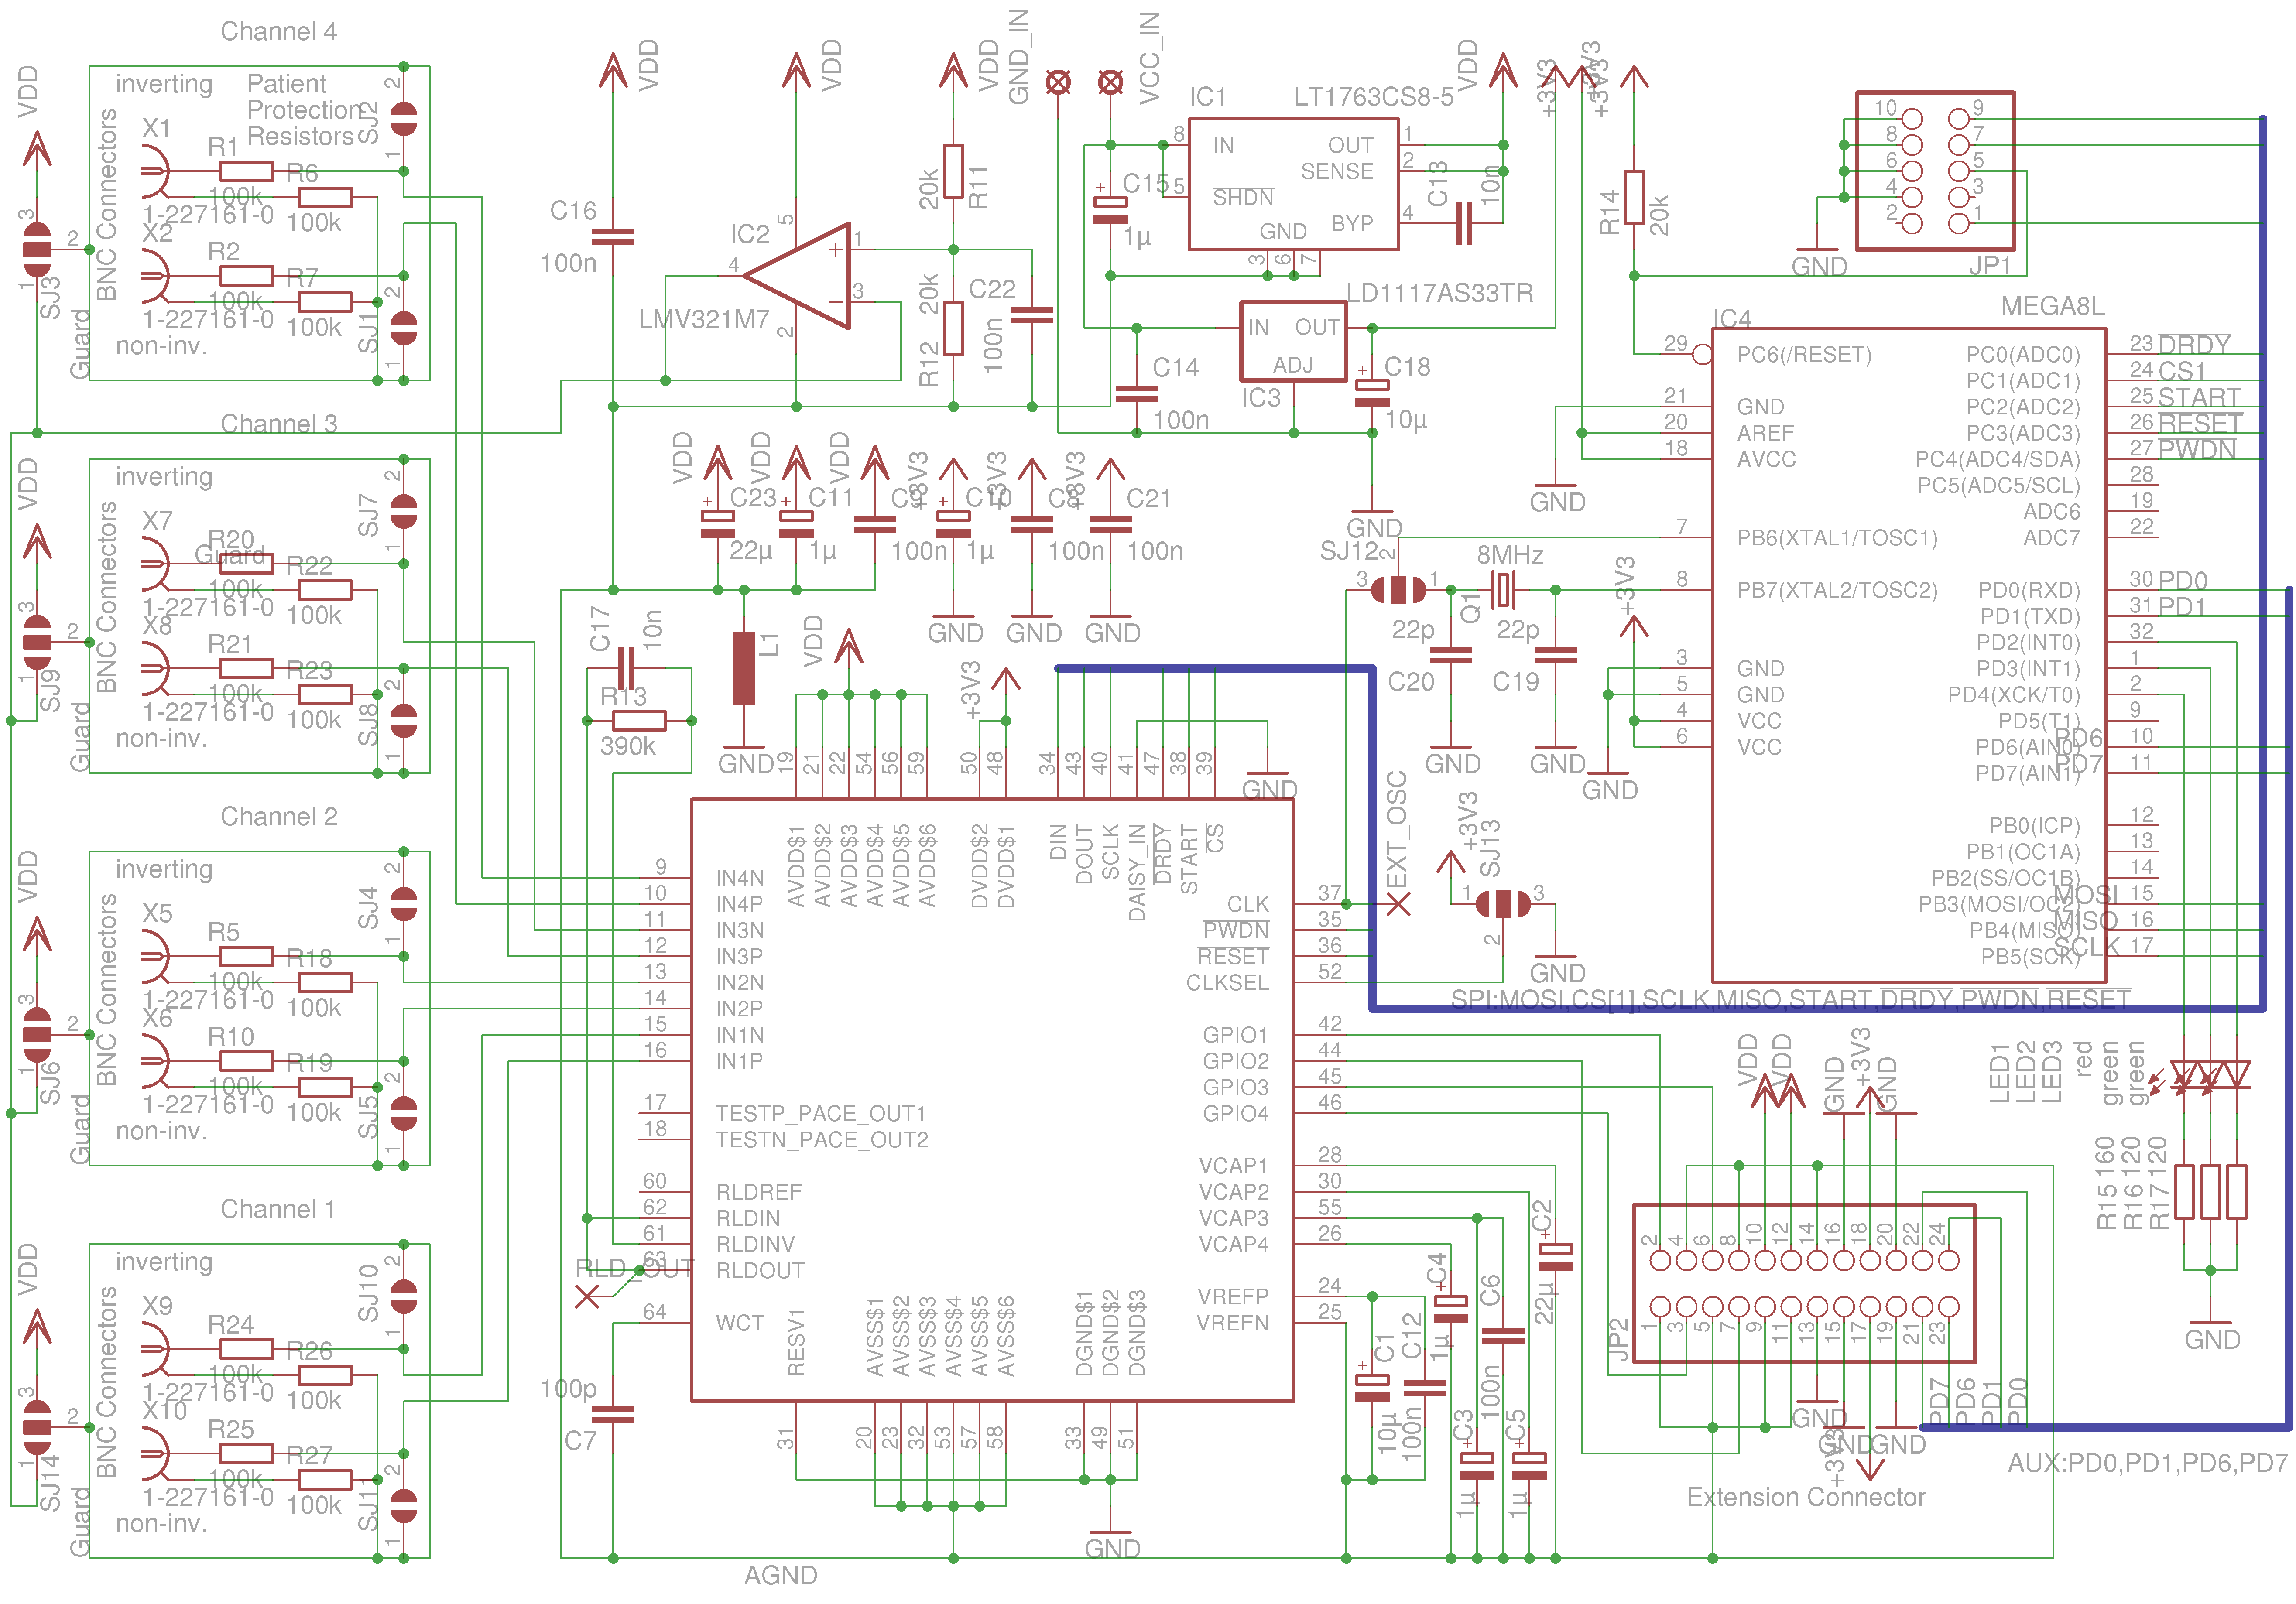
\includegraphics{images/adc_schematic_01.png}
\label{adc_schematic}
\caption{Der Schaltplan des EEG-Moduls}
\end{figure}
\end{landscape}

\newglossaryentry{Sampling}{name={Sampling}, description={Umwandlung eines kontinuierlichen, meist analogen Signals in diskrete Werte und -- im Falle eines ADC oder DAC -- die Umwandlung desselben in digitale Signale}}
\newglossaryentry{Nyquist-Theorem}{name={Nyquist-Theorem}, description={}}
\newglossaryentry{Offsetkorrektur}{name={Offsetkorrektur}, description={}}
%TODO: gls entries
Die \gls{Sampling}-Rate liegt im Bereich einiger hundert bis tausend $\frac{Sp}{s}$, die höchste für die Messung signifikante Frequenz liegt weit unter $100Hz$. Das \glslink{Nyquist-Theorem}{Nyquist-Shannonsche Abtasttheorem} ist somit erfüllt und bei den gegebenen Frequenzen sind keine Probleme zu erwarten.
Die Auflösung des \gls{ADC} ist mit 16 Bit groß genug, um \gls{Offsetkorrektur} und weitere Filtermaßnahmen in Software zu implementieren, wodurch keine weiteren analogen eingangsseitigen Filter notwendig sind.
%Quelle: Nyquist

%BEGIN OF TODOS
% --- PAPER ---
%Include: in the PWM section: Duty cycle
% --- SOURCES ---
%AN4348 Pg. 5: Error? The tolerance calculation seems to be mixing up ppms and percents.
% --- ELECTRONICS ---
%Incorporate a MAX5490 or similar calibrated R-R ladder as reference voltage divider
%Input decoupling necessary?
%END OF TODOS
\subsection{Mathematisch und Informatisch}
\section{Arbeitsprozess der Platinenherstellung und Ergebnisse}
\appendix
\section{Glossar}
%FIXME
\glsaddall
\printglossaries
\section{Literatur, Quellen etc.}
\nocite{*}
\bibliographystyle{plain}
\renewcommand{\refname}{}
%TODO \footnotesize
\bibliography{rgbulb}
\section{Updates}
\begin{center}
\Ovalbox{
\begin{minipage}{11cm}
\begin{center}
\sffamily%\color{red}
\vspace{2mm}
Die jeweils aktuellte Version dieser Arbeit, der Quelltexte und der Hardwaredokumentation ist unter der Adresse 
\url{http://github.com/jaseg/RGBulb} zu finden. Die Repositories der einzelnen Unterprojekte sind unter den folgenden Adressen zu finden:
\begin{description}
\item \url{https://github.com/jaseg/OpenMind}
\item \url{https://github.com/jaseg/BUZ2-Master}
\item \url{https://github.com/jaseg/BUZ2-Slave}
\end{description}
\vspace{2mm}
\end{center}
\end{minipage}
}
\end{center}
\section{Changelog}
\begin{tabularx}{\textwidth}{l|l}
\textbf{Version}&\textbf{Anmerkungen}\\\hline
0.1&Arbeitsversion
\end{tabularx}
\end{document}